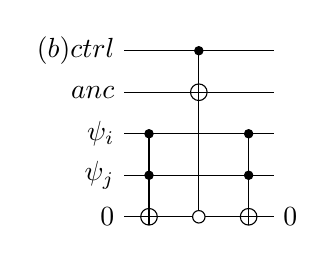
\begin{tikzpicture}[scale=1.000000,x=1pt,y=1pt]
\filldraw[color=white] (0.000000, -7.500000) rectangle (54.000000, 67.500000);
% Drawing wires
% Line 1: ctrl W \text{(b) }ctrl
\draw[color=black] (0.000000,60.000000) -- (54.000000,60.000000);
\draw[color=black] (0.000000,60.000000) node[left] {$\text{(b) }ctrl$};
% Line 2: anc W anc
\draw[color=black] (0.000000,45.000000) -- (54.000000,45.000000);
\draw[color=black] (0.000000,45.000000) node[left] {$anc$};
% Line 3: i W \psi_i
\draw[color=black] (0.000000,30.000000) -- (54.000000,30.000000);
\draw[color=black] (0.000000,30.000000) node[left] {$\psi_i$};
% Line 4: j W \psi_j
\draw[color=black] (0.000000,15.000000) -- (54.000000,15.000000);
\draw[color=black] (0.000000,15.000000) node[left] {$\psi_j$};
% Line 5: clean0 W 0 0
\draw[color=black] (0.000000,0.000000) -- (54.000000,0.000000);
\draw[color=black] (0.000000,0.000000) node[left] {$0$};
% Done with wires; drawing gates
% Line 7: i j +clean0
\draw (9.000000,30.000000) -- (9.000000,0.000000);
\filldraw (9.000000, 30.000000) circle(1.500000pt);
\filldraw (9.000000, 15.000000) circle(1.500000pt);
\begin{scope}
\draw[fill=white] (9.000000, 0.000000) circle(3.000000pt);
\clip (9.000000, 0.000000) circle(3.000000pt);
\draw (6.000000, 0.000000) -- (12.000000, 0.000000);
\draw (9.000000, -3.000000) -- (9.000000, 3.000000);
\end{scope}
% Line 8: -clean0 ctrl +anc
\draw (27.000000,60.000000) -- (27.000000,0.000000);
\draw[fill=white] (27.000000, 0.000000) circle(2.250000pt);
\filldraw (27.000000, 60.000000) circle(1.500000pt);
\begin{scope}
\draw[fill=white] (27.000000, 45.000000) circle(3.000000pt);
\clip (27.000000, 45.000000) circle(3.000000pt);
\draw (24.000000, 45.000000) -- (30.000000, 45.000000);
\draw (27.000000, 42.000000) -- (27.000000, 48.000000);
\end{scope}
% Line 9: i j +clean0
\draw (45.000000,30.000000) -- (45.000000,0.000000);
\filldraw (45.000000, 30.000000) circle(1.500000pt);
\filldraw (45.000000, 15.000000) circle(1.500000pt);
\begin{scope}
\draw[fill=white] (45.000000, 0.000000) circle(3.000000pt);
\clip (45.000000, 0.000000) circle(3.000000pt);
\draw (42.000000, 0.000000) -- (48.000000, 0.000000);
\draw (45.000000, -3.000000) -- (45.000000, 3.000000);
\end{scope}
% Done with gates; drawing ending labels
\draw[color=black] (54.000000,0.000000) node[right] {$0$};
% Done with ending labels; drawing cut lines and comments
% Done with comments
\end{tikzpicture}
